\subsection{Magic Cube}
A \mcube{} is created from squares put on top of each other so they make up a cube form. 
This makes it clear that there is a connection between \msquare{}s and  \mcube{}s.
An example of this can be seen on figure \ref{fig:presentMagicCube}.

\begin{figure}[h]
	\centering
		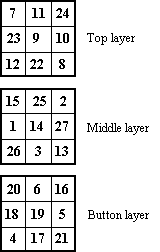
\includegraphics[scale=0.8]{input/pics/presentMagicCube}
	\caption{\myCaption{This is a magic cube split up into 3 magic squares.}}
	\label{fig:presentMagicCube}
\end{figure}

Both of them have a magic constant, which can be the sum of each row, colon and diagonal if it is a  \mcube{} or normal \msquare{}.
This i where the similarity ends.

We have shown how to calculate the magic constant in a \msquare{}.
In a  \mcube{} there is not a big difference in the formula to calculate the magic constant.
\begin{equation}
	M(n)=\frac{n \cdot (n^3+1)}{2}
\end{equation}
As shown in the formula the only difference is the power of $n$ that is changed from 2 to 3.
This will be show in appendix \ref{sec:proofOfMagicConstant} why it is so.

To create a  \mcube{}, there are some parts that needs to be explanied.
All these basics are shown on figure \ref{fig:cubeparts}.

\begin{figure}[h]
	\centering
		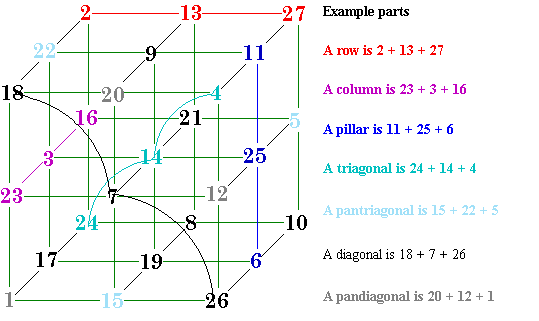
\includegraphics[scale=0.3]{input/pics/cubeparts}
	\caption{\myCaption{This is a Magic Cube where the colors show all of the parts.}}
	\label{fig:cubeparts}
\end{figure}

Because of all these different parts there are a lot of different ways to define  \mcube{}s.
The simplets of them all is a simpel  \mcube{}, the only requirements to make such a cube is the following:
\begin{itemize}
	\item All 9- rows, columns and pillars must equal the magic constant.
	\item All 4 triagonals must also equal the magic constant.
\end{itemize}

\begin{figure}[h]
	\centering
		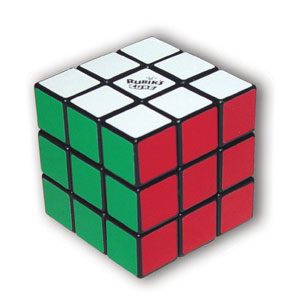
\includegraphics[scale=0.4]{input/pics/rubiksCube}
	\caption{This is a Rubiks Cube.}
	\label{fig:rubiksCube}
\end{figure}

When looking at the \rubik{} it is easy to see that it looks a lot like the \mcube{}. There are two differences one is that the \mcube{} has a number in the center where the \rubik{} do not because it is rotating around the center. The other difference is that the \mcube{} consist of numbers whereas the \rubik{} have colors, which are diffent on each \face{}s.
